% Preamble
\documentclass[11pt]{article}

% Packages
\usepackage{a4wide}
\usepackage{graphicx}
\usepackage{url}
\graphicspath{{images/}}
\usepackage[nottoc]{tocbibind}
\usepackage{listings}
\usepackage{caption}
\usepackage{amsmath}

% Author
\author{Van Dam, Thijs\\
\and
Bos, Sander\\
}
\title{\huge The Animal Kingdom}
\date{April 2018}

\setlength{\parindent}{0em}
\setlength{\parskip}{1em}

\DeclareCaptionFormat{cancaption}{#1#2#3\par}
\DeclareCaptionLabelFormat{cancaptionlabel}{#1}
\captionsetup[figure][number]{format=cancaption,labelformat=cancaptionlabel}

% Document

\begin{document}
    \maketitle
    \thispagestyle{empty}
    \newpage
    \newpage
    \setcounter{page}{1}
    \section{Introduction}\label{sec:introduction}
    \begin{itemize}
        \item Steering
        \item Path planning
        \item Behaviour
        \item Fuzzy logic
    \end{itemize}

    \newpage
    \tableofcontents
    \newpage
    %-----------------------------------------------------------------------------------------
    \section{Steering}\label{sec:steering}

    \newpage
    %-----------------------------------------------------------------------------------------
    \section{Path planning}\label{sec:pathPlanning}
    This section contains all information about the path planning algorithms and structure used in 'The Animal Kingdom'.
    \subsection{Structure}\label{subsec:pathstructure}
    Buckland\cite{pgaie} describes a well-structured approach to splitting logic for the pathfinding.
    This same structure is what we used in our application, although we have made some changes to fit our own needs.
    The application contains one instance of a \textit{PathManager} and each (moving) entity contains a \textit{PathPlanner}.
    The \textit{PathPlanner} is what is used to request a new search with the specified algorithm (A* or Dijkstra).
    When a request is done, the \textit{PathPlanner} registers itself in the \textit{PathManager}.
    Using a \textit{PathManager} makes it possible to manage and control all search requests from one place.
    This is especially useful when you want to implement time-slicing or other logic that restricts the amount of search cycles per update.
    The latter case is what we use it for.
    \textit{PathManager} contains a function \textit{UpdateSearches()} which lets each \textit{PathPlanner} do one or more cycle depending on the maximum cycles set while instantiating the \textit{PathManager}.
    What a cycle does, will be discussed in section \ref{subsec:pathalgorithms}.\par
    The class diagram below shows the structure of the pathfinding logic including the \textit{PathManager} and \textit{PathPlanner}.

    \begin{figure}[h!]

        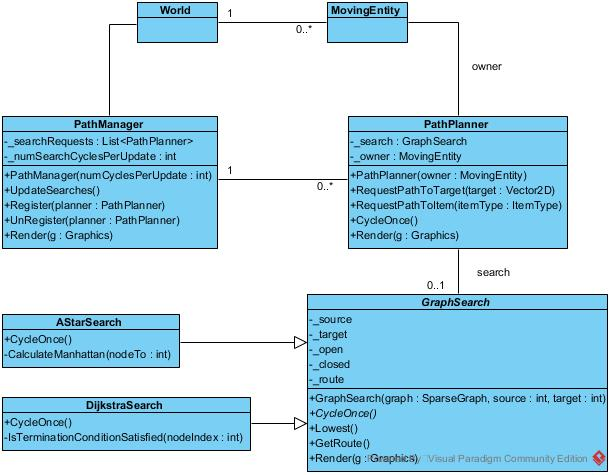
\includegraphics[width=30em]{PathFinding.jpg}

        \caption{Path planning class diagram}

        \label{fig:pathPlanClassDiagram}

    \end{figure}
    
    \subsection{Creating a graph}\label{subsec:pathgraphcreation}
    The graph in the game world is created using a floodfill.
    A single point is given as its starting position and from that point edges and nodes are added in every direction.
    If the placing of an edge or node is obstructed by an obstacle, it will not be created and the floodfill will continue
    in the other directions.
    This results in a graph that fills the complete game world.
    The graph itself is not saved as a file, it is possible to do this, but because of the small area of the field,
    generating a graph at the start of the application doesn't affect performance and loading time.
    The picture below (see fig.\ref{fig:pathPlanFloodfill}) demonstrates the result of using floodfill.

    \begin{figure}[h!]

        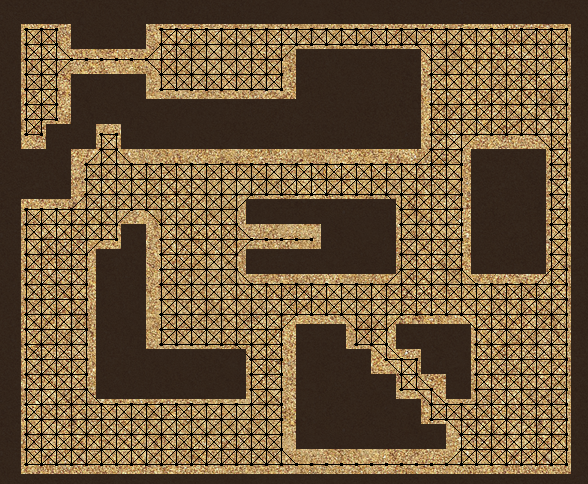
\includegraphics[width=30em]{Floodfill.jpg}

        \caption{The result of using floodfill}

        \label{fig:pathPlanFloodfill}

    \end{figure}
    
    \subsection{Algorithms}\label{subsec:pathalgorithms}
    As mentioned previously, we have implemented two path-finding algorithms in the application.
    Dijkstra and A*. Each of the algorithms is implemented in a separate class extending the \textit{GraphSearch} class.
    Both implementations will be discussed below.
    
    \subsubsection{Dijkstra}\label{sec:pathDijkstra}
    The first algorithm we implemented, is Dijkstra as it is also the base of the A* algorithm.
    Although the algorithm was already familiar to us, implementing it was a bit more difficult than we expected.
    It was not a lot of work, but it did require some thinking.
    In Programming Game AI by Example, Buckland describes a version of the algorithm that looked more complex than necessary.
    Luckily we found a pseudo code\cite{aapc} of A*, which by removing the heuristics, was a much better understandable version of the algorithm.\par
    
    A first version of the algorithm was without the \textit{PathManager} and/or \textit{PathPlanner} and did not contain the \textit{CycleOnce()}.
    Instead, we had a single function \textit{Search()} which did the whole search at once.
    The function \textit{IsTerminationConditionSatisfied()} was added to check if an item of the specified \textit{ItemType} was found.
    If a matching item was found, the algorithm was stopped and the route was returned.
    The resulting route was eventually drawn on the screen by adding a \textit{Render()} function.
    
    \subsubsection{A*}\label{sec:pathAstar}
    As A* is basically Dijkstra with heuristics, it was easy to convert our existing Dijkstra algorithm to A*.
    Just as with the Dijkstra algorithm, we first created a single \textit{Search()} which did the whole search at once.
    The heuristic used for our implementation is Manhattan, which we calculated in \textit{CalculateManhattan()}.
    The distance between all nodes is the same in the graph and each edge has a cost of 1.
    Calculating the Manhattan distance was very easy as we could just calculate the distance between the current node and target location
    and devide it by the length of one edge to get the estimated distance (see fig.\ref{fig:pathPlanCalcManhattan}).

    \begin{figure}[h!]

        \[ $$M = \dfrac{|targetLocation.X - currentLocation.X| + |targetLocation.Y - currentLocation.Y|}{15}\]

        \caption{Calculating the Manhattan distance}

        \label{fig:pathPlanCalcManhattan}

    \end{figure}
    
    
    \subsection{Performance}\label{subsec:pathperformance}
    Because of the implementation of the \textit{PathManager} and \textit{PathPlanner} resources will be shared equally between all moving entities.
    There is also a predifined maximum amount of calculation cycles per update, which prefents the game from slowing down.
    At first we struggled with this, as it seemed to take much longer to find a path than previoulsy with just the single \textit{Search()} function.
    After a bit of tweaking (changing the maximum amount of cycles per update) and removing a lot of \lstinline[columns=fixed]{Console.WriteLine(...)}
    lines used for debugging which were clearly slowing down the calculations as they were limited by the speed of the console.\par
    
    However, performance can still be improved.
    Storing precalculated costs, or some shortest paths could dramatically improve the performance when the amount of agents increases.
    
    \newpage
    %-----------------------------------------------------------------------------------------
    \section{Behaviour}\label{sec:behaviour}
    
    \newpage
    %-----------------------------------------------------------------------------------------
    \section{Fuzzy logic}\label{sec:fuzzyLogic}

    \newpage
    %-----------------------------------------------------------------------------------------
    \section{Conclusion}\label{sec:conclusion}

    \newpage
    %-----------------------------------------------------------------------------------------

    \bibliographystyle{unsrt}
    \bibliography{sources}
\end{document}